% This is "sig-alternate.tex" V2.0 May 2012
% This file should be compiled with V2.5 of "sig-alternate.cls" May 2012
%
% This example file demonstrates the use of the 'sig-alternate.cls'
% V2.5 LaTeX2e document class file. It is for those submitting
% articles to ACM Conference Proceedings WHO DO NOT WISH TO
% STRICTLY ADHERE TO THE SIGS (PUBS-BOARD-ENDORSED) STYLE.
% The 'sig-alternate.cls' file will produce a similar-looking,
% albeit, 'tighter' paper resulting in, invariably, fewer pages.
%
% ----------------------------------------------------------------------------------------------------------------
% This .tex file (and associated .cls V2.5) produces:
%       1) The Permission Statement
%       2) The Conference (location) Info information
%       3) The Copyright Line with ACM data
%       4) NO page numbers
%
% as against the acm_proc_article-sp.cls file which
% DOES NOT produce 1) thru' 3) above.
%
% Using 'sig-alternate.cls' you have control, however, from within
% the source .tex file, over both the CopyrightYear
% (defaulted to 200X) and the ACM Copyright Data
% (defaulted to X-XXXXX-XX-X/XX/XX).
% e.g.
% \CopyrightYear{2007} will cause 2007 to appear in the copyright line.
% \crdata{0-12345-67-8/90/12} will cause 0-12345-67-8/90/12 to appear in the copyright line.
%
% ---------------------------------------------------------------------------------------------------------------
% This .tex source is an example which *does* use
% the .bib file (from which the .bbl file % is produced).
% REMEMBER HOWEVER: After having produced the .bbl file,
% and prior to final submission, you *NEED* to 'insert'
% your .bbl file into your source .tex file so as to provide
% ONE 'self-contained' source file.
%
% ================= IF YOU HAVE QUESTIONS =======================
% Questions regarding the SIGS styles, SIGS policies and
% procedures, Conferences etc. should be sent to
% Adrienne Griscti (griscti@acm.org)
%
% Technical questions _only_ to
% Gerald Murray (murray@hq.acm.org)
% ===============================================================
%
% For tracking purposes - this is V2.0 - May 2012

\documentclass{sig-alternate}
\usepackage{epstopdf}
\usepackage{epsfig}
%\usepackage{fontspec} 
%\setmainfont{URW Palladio L}
%\newfontfamily\jap[Scale=0.8]{Kochi Mincho}  % here we simply define a new font switch
%\usepackage{xltxtra}
\usepackage{CJK}
\epstopdfsetup{suffix=-\SourceExt-converted-to}
\usepackage{algpseudocode}
\usepackage{algorithmicx}

\begin{document}
%
% --- Author Metadata here ---
\conferenceinfo{CEA2013}{Barcelona, Catalunya, Spain, October 21, 2013}
%\CopyrightYear{2007} % Allows default copyright year (20XX) to be over-ridden - IF NEED BE.
%\crdata{0-12345-67-8/90/01}  % Allows default copyright data (0-89791-88-6/97/05) to be over-ridden - IF NEED BE.
% --- End of Author Metadata ---

\title{A Regional Food's Features Extraction Algorithm and Its Application}

%
% You need the command \numberofauthors to handle the 'placement
% and alignment' of the authors beneath the title.
%
% For aesthetic reasons, we recommend 'three authors at a time'
% i.e. three 'name/affiliation blocks' be placed beneath the title.
%
% NOTE: You are NOT restricted in how many 'rows' of
% "name/affiliations" may appear. We just ask that you restrict
% the number of 'columns' to three.
%
% Because of the available 'opening page real-estate'
% we ask you to refrain from putting more than six authors
% (two rows with three columns) beneath the article title.
% More than six makes the first-page appear very cluttered indeed.
%
% Use the \alignauthor commands to handle the names
% and affiliations for an 'aesthetic maximum' of six authors.
% Add names, affiliations, addresses for
% the seventh etc. author(s) as the argument for the
% \additionalauthors command.
% These 'additional authors' will be output/set for you
% without further effort on your part as the last section in
% the body of your article BEFORE References or any Appendices.

\numberofauthors{3} %  in this sample file, there are a *total*
% of EIGHT authors. SIX appear on the 'first-page' (for formatting
% reasons) and the remaining two appear in the \additionalauthors section.
%
\author{
% You can go ahead and credit any number of authors here,
% e.g. one 'row of three' or two rows (consisting of one row of three
% and a second row of one, two or three).
%
% The command \alignauthor (no curly braces needed) should
% precede each author name, affiliation/snail-mail address and
% e-mail address. Additionally, tag each line of
% affiliation/address with \affaddr, and tag the
% e-mail address with \email.
%
% 1st. author
\alignauthor
Trung Duc Nguyen \\
       \affaddr{Falcuty of Enviroment and Information Study}\\
       \affaddr{Keio University, Fujisawa, Kanagawa, Japan}\\
       \email{deplop@wide.sfc.ad.jp}
% 2nd. author
\alignauthor
Diep Thi-Ngoc Nguyen\\
       \affaddr{Graduate School of Media and Governance}\\
       \affaddr{Keio University, Fujisawa, Kanagawa, Japan}\\
       \email{chupi@sfc.keio.ac.jp}
% 3rd. author
\alignauthor 
Yasushi Kiyoki\\
       \affaddr{Graduate School of Media and Governance}\\
       \affaddr{Keio University, Fujisawa, Kanagawa, Japan}\\
       \email{kiyoki@sfc.keio.ac.jp}
}

\maketitle
\begin{abstract}
 
%Advantages
Automatically detecting food's taste is a non-trivial part. However, we realize that the taste of food can be extracted by directly analyzing recipes by the ingredients and the amount of them in the recipes. 
In this paper, we present a food analysis system to discover the taste of foods and to better understand the featured ingredients in each specific geographical region. The main features of this system are (1) to extract dominant ingredients and tastes in a region by analyzing the ingredients' frequency and its uniqueness, and (2) to transform user's existing materials or original recipe to a new recipe according to a targeted taste. To examine the feasibility and applicability of the algorithm, we have developed a web-based application with a recipe database collected from approximately 200 recipes in over 7 regions of Japan: Hokkaido-Tohoku, Kanto, Kansai, Shikoku, Tyubu, Kyusyu-Okinawa and Tyugoku. 
 
\end{abstract}

% A category with the (minimum) three required fields
\category{H.4}{Information Systems Applications}{Miscellaneous}


\terms{Algorithm, Experimentation}

\keywords{recipe retrival, text mining, web crawler, dynamic recipe, food's features}

\section{INTRODUCTION}
In this paper, we present a food analysis system to discover the taste of food and understand the featured ingredients in a specific geographical region.
%Background
\par Cooking is the art of making foods. Nowadays, together with the development of technology and the availability of equipment in cooking, many supporting systems are introduced. For example, the cooking support system utilizing built-in cameras and projectors~\cite{morioka:camera-projecter}, the cooking support system by using ubiquitous sensors~\cite{nakauchi:recog}, the calorie measurement system by image processing~\cite{villalobos:image-calorie} or the system which helps inexperienced users in understanding non-professional recipe descriptions~\cite{ide:inexper}, etc. However, by using analysis job we can discover the dominant ingredients and tastes in foods and understand how to alter the taste from one to another.
%The problem statement
\par We can observe that in geographical regions that are far apart from each other often have different features and tastes. For example, the Kanto region, which is located in the East of Japan, often has dense taste in its foods, while the foods in Kansai region, which lies in the southern-central region of Japan's main island Honshu, often has a diluted taste. The reason is because each region has its own special materials for foods and people in these regions have different habits in cooking food. To understand each region's featured taste we need to answer the following questions: ``How can we understand the different features of each region's food?'' and ``What effects change the region's food taste?''. Among the many factors that affect a food's taste, the combination of materials is a direct and important factor. Each recipe has a list of its own ingredients together with their amount. This leads us to the idea that we could automatically achieve the features of a region's foods by analyzing the materials. In order to make advantages of recipes in food analysis, we collected recipes in many regions to build a recipe database and propose some analysis algorithms based on text processing.

%The need of the system
\par We also realize that understanding the region's featured taste and the preferred materials has an application in supporting cooking activities. For example, imagine someone living in Kanto region who wants to eat some traditional foods in the Kansai region. They know the original recipe but there are some tastes in Kansai region that are not favored. They would prefer that traditional foods with replaced ingredients that are easy for Kanto people to eat. Conversely, someone living in Kanto region might want to try Kanto foods with Kansai taste. Solving this kind of problem means we can build up a system which can help people satisfy their taste. The recipes, which are made by the system, would be flexible and diverse.
%Approach 
\par In the existing cooking support systems, the methods vary such as image processing, text retrieval, sensing, etc. We use the text processing approach to directly analyze the recipes with their ingredients and amount of ingredients. 
%Outline
\par The outline of this paper is as following. The algorithm and the experimental results are introduced in Section 2 and Section 3 respectively. Section 4 describes the web-based application using the proposed algorithm while Section 5 concludes and discusses the remaining problems and future works. 
 
 
\section{region's featured materials analyzing algorithm}

In this section, we propose an algorithm for analyzing the dominant materials which are often used in a region. We define a material in a region to be a featured one if it appears many times with a large amount and be unique among recipes in that region. To evaluate whether it is featured or not, we suppose that the following questions should be answered: ``How often, how much, and how unique the material is?''. Respectively, we propose three kind of functions to answer these questions. They have the key role of the metrics for the featured ingredient's evaluation.  

\subsection{Ingredient Frequency}

The first function named $IF$ (Ingredient Frequency) is used to treat the question ``How often does the material appear in a region?''. The higher frequency an ingredient appears in a region, the higher possibility it is the region's featured ingredient. In each recipe, an ingredient only appears one time. Thus, the time that ingredient appears in the region is the number of the recipes in the region has it as ingredient. Because the database we have from the Internet are often unbalanced, there are some regions that have more recipes than others. Thus to make it indenpendent from the database, we prefer to use the ingredient's frequency rather than its appearance times. This function is formed by the number of times the ingredient appears in the region's recipes over the number of total recipes in that region.

Let $R$ be the set of all recipes ($r$) in a region and $i$ be an ingredient which appears in the region. The function is formed as follows:
\begin{center}
\smallskip
$ IF(i,R)= \frac{\displaystyle | \{i | i \in r, r \in R \} | }{\displaystyle | R | }$
\smallskip
\end{center}


Becaue the $IF$ value is the ingredient's frequency, it takes the value between 0 and 1.

\subsection{Ingredient Amount}

The ingredient's frequency has little meaning if there is a small amount of it in the recipes. Thus, the taste of a food not only depends on the ingredients, but also the amount of the ingredients. Even when an ingredient has a high value of $IF$, it might not be the region's featured ingredient. Thus, the second function, $IA$, is proposed for the question ``How much?''

Let $r$ be a recipe in the set of recipes $S$ and ingredient $i$ is in $r$. 
We define the mean function $M(i,S)$ be the mean amount of $i$ in $S$ as follows: 
\begin{center}
\smallskip
$M(i,S)= \frac{\displaystyle \sum_{}^{i \in r, r \in S} amount(i,r)}{\displaystyle |\{i|i \in r, r \in S\}|}$
\smallskip
\end{center}

in which $amount(i,r)$ is the amount of ingredient $i$ in recipe $r$.

We also assume that $AR$ is the set of all recipes in the country regardless of the region it belongs to, while $R$ is the set of all recipes just in a specific region. Thus, $M(i,R)$ calculates the mean amount of ingredient $i$ in the region's recipes ($R$) while $M(i,AR)$ calculate the mean amout of ingredient $i$ in all the country's recipes ($AR$). We have the $IA$ function as follows:
\begin{center}
\smallskip
$IA(i,R)= \frac{\displaystyle M(i,R)}{\displaystyle M(i,AR)}$
\smallskip
\end{center}


Because the $IA$ function calculates the mean of ingredient's amount, it is independent to the frequency of that ingredient. The higher $IA$ value is, the higher possibility it is the region's featured ingredient. Because both numerator and denominator in the formula have the same unit, the $IA$ value is non-unit. Therefore, regardless to the variety of the ingredient's unit, we have a stable metric for evaluating the ingredient's amount.

\subsection{Ingredient Unique}

The $IF$ and $IA$ functions above might tell us how often an ingredient appears in the region, but this ingredient can often appear in many regions. To be a featured ingredient of a region, the ingredient must satisfy the condition that it appears in the region but doesn't appear in many other regions. We propose the third function $IU$ as follows: 
\begin{center}
\smallskip
$IU(i,A)=  \log{\displaystyle \frac{\displaystyle |A|}{\displaystyle |\{i|i \in a, a \in A \}|}}$
\smallskip
\end{center}

in which $i$ is the ingredient in region $a$ and $A$ is the set of regions.

This function calculates the uniqueness of an ingredient among all the regions. The more often an ingredient appears in different regions the less unique it is. In other words, it is not the featured ingredient of the region. The higher $IU$ value corresponds to higher possibility it is the region's featured ingredient. We use the log scale to make sure the $IU$ values are not too big.

\subsection{Featured Index}

Featured Index, which is denoted by $FI$, is the index used to rank ingredients in a region in term of featured ingredient. We realize that these three functions are all proportional to the rank of the featured ingredient, thus we proposed $FI$ to be the production of these three function's values as follows.
\begin{center}
\smallskip
$FI(i,R)= IF(i,R) \times IA(i,R) \times IU(i,A)$ 
\smallskip
\end{center}

The $FI$ function returns the featured index of ingredient $i$ in a region which has a set of recipes $R$. $A$ is the set of all regions in the country. The ingredients which have the highest $FI$ would be the featured ingredients. On the other hands, the ingredients which have the lowest $FI$ would be considered as the common ingredients for every region.

\section{Experiment on regional food feature analysis}

This section describes the recipe databse and experimental studies on this database by applying the featured ingredient analysis algorithm.  

\subsection{The Recipe Database}

We build a recipe database in which recipes are grouped by region. A script written in Python crawls all the recipes from a Japanese cooking website~\cite{web:recipe}. We chose this website because the recipes are typical foods grouped by regions. The website is only for Japanese recipes, thus we now only have the database for Japanese foods. Each food is characterized by its name, the region it belongs to and its recipe. Each recipe is stored as a map collection in which the ingredient is the key and the couple of amount and unit is the value. Each of the recipes we get from the website is created for various amounts of people. For example, there are recipes for 4 people but there are also recipes for 3 people. Thus we need to normalize the ingredients' amount in each recipe for one person.

\par There are about 200 recipes over 7 regions in Japan: Kanto, Hokkaido-Tohoku, Shikoku, Tyubu, Kyusyu-Okinawa, Kansai and Tyugoku. We calculate all the above functions for every recipe in Japan, but we only show the experimental results of Kanto and Shikoku within this paper. We chose these two regions because they lie far apart in different islands of Japan. The experimental results are discussed below. 

\subsection{Ingredient Frequency}

\begin{CJK}{UTF8}{min}

Table~\ref{tab:IF} shows that there are some common ingredients which often appear in both Kanto and Shikoku regions such as Soy Sauce (しょうゆ), Sake (酒), Salt (塩),\ldots This is reasonable because we know that these ingredients are common in Japan. Because they often appear in other regions, the $IF$ function is not enough to evaluate the region's featured ingredients. However, it helps us partially understand the habit in using materials in regions. For example, Green onion (万能ねぎ) often appears in Shikoku but not in Kanto region and Sugar (砂糖) often appears in Kanto but not in Shikoku region. This leads us to the idea that typical Kanto foods are often sweeter than Shikoku foods. 

\begin{table}

\centering
\caption{Ingredient Frequency of Ingredients in Kanto region vs Shikoku region}
\begin{tabular}{|c|c|c|c|}
\hline
\multicolumn{2}{|c|}{\textbf{\large Kanto region}} & \multicolumn{2}{|c|}{\textbf{\large Shikoku region}} \\
\cline{1-4}

\textbf{Ingredient} &\textbf{ IF} & \textbf{Ingredient} & \textbf{IF}\\ \hline
Soy Sauce (醤油) 	& 1.00 & Soy Sauce (醤油) & 1.00 \\ \hline
Miso (みそ)			& 0.9  &	 Salt (塩)	& 1.00  \\ \hline
Sugar (砂糖) 			& 0.83 & Rice (米) & 0.83 \\ \hline
Sake (酒)				& 0.83 & Sake (酒) & 0.67\\ \hline
Salt 			& 0.67 & Green onion & 0.50\\
(塩) & & (万能ねぎ) & \\ \hline
\ldots &\ldots & \ldots & \ldots \\ \hline
Dried bonito  			& 0.08 	& Kelp soup 	& 0.16  \\ 
(かつお節) & & (ダシ昆布) & \\ \hline
Pumpkin 			& 0.08 & Deep-fried Tofu 	& 0.16  \\ 
(かぼちゃ)  & & (油揚げ) & \\ \hline
Kamaage Shirashi  & 0.08 & Seared bonito  & 0.16  \\ 
(釜揚げしらす)  & & (鰹の敲き) & \\\hline		

\end{tabular}

\label{tab:IF}
\end{table}

\end{CJK}


\subsection{Ingredient Amount}

\begin{CJK}{UTF8}{min}

\begin{table}

\centering
\caption{Ingredient Amount of Ingredients in Kanto region vs Shikoku region}
\begin{tabular}{|c|c|c|c|}
\hline
\multicolumn{2}{|c|}{\textbf{\large Kanto region}} & \multicolumn{2}{|c|}{\textbf{\large Shikoku region}} \\
\cline{1-4}

\textbf{Ingredient} &	\textbf{IA} &\textbf{Ingredient} & \textbf{IA}\\ \hline
White radish & 4.27 &  Shredded seaweed& 6.00 \\
(大根)	& &  (刻みのり)  & \\ \hline
Tempura flour 	& 3.20  & Carrot& 3.95 \\
(天ぷら粉)  & &  (にんじん) & \\ \hline
 Shredded seaweed 		& 3.00 & Tempura flour & 3.20\\
(刻みのり) & &  (天ぷら粉)  & \\ \hline
\ldots &\ldots & \ldots & \ldots \\ \hline
Taro 	& 0.02& Sweet potato &0.06 \\ 
 (里芋)	&  &  (さつまいも) & \\ \hline
Cake flour	& 0.02& Chicken thigh&0.05\\ 
 (薄力粉) & &  (鶏もも肉) & \\ \hline
Field mustard	& 0.02& Sushi vinegar & 0.05\\
 (菜の花)  & & (すし酢) & \\ \hline

\end{tabular}

\label{tab:IA}
\end{table} 
 
Table~\ref{tab:IA} shows the result of the $IA$ value for Kanto and Shikoku region. We can see that most of the $IA$ values are around 1, which means there is not much difference in the way of using an ingredients' amount between Shikoku region and other regions. However, there are some interesting results. For example, in Kansai region, the mean amount of pepper (こしょう) is 11 times greater than the mean amount of total peper in Japan. See details in Table~\ref{tab:IAoutlier}. 




\subsection{Ingredient Uniqueness}
\begin{CJK}{UTF8}{min}

Table~\ref{tab:IU} reflects the fact that the common ingredients such as Salt (塩), Sweet cooking wine (みりん), Ginger (しょうが), Soy sauce (しょうゆ) appear in almost every regions in Japan while the ingredients such as Peanut (落花生) and Chive (あさつき) are not too common and mostly appear in only one region. The ingredients which have the $IU$ value of 0 appear in every region.


\begin{table}
\centering
\caption{Ingredient Amount of Ingredients in Tyubu region vs Kansai region}
\begin{tabular}{|c|c|c|c|}
\hline
\multicolumn{2}{|c|}{\textbf{\large Tyubu region}} & \multicolumn{2}{|c|}{\textbf{\large Kansai region}} \\
\cline{1-4}

\textbf{Ingredient} &\textbf{ IA} & \textbf{Ingredient} & \textbf{IA}\\ \hline
Pork loin 	&	25.50 	& Pepper 	&11.00\\ 
 (豚ロース肉) & & (こしょう) & \\ \hline
Seaweed 		&	6.00		& Sweet cooking wine 		&6.88\\ 
(刻みのり) & & (みりん) & \\ \hline
Green onion 	&	3.72		& Soy sauce 	& 5.49\\ 
 (長ねぎ)	 & & (醤油)	 & \\ \hline
Onion		&	3.60		& Green onion 		&3.72\\ 
 (玉ねぎ) & & (長ねぎ) & \\ \hline
\ldots &\ldots & \ldots & \ldots \\ \hline
Taro (里芋)			&	0.03		& Milk (牛乳)		&0.04\\ \hline
Cake flour	&	0.02		& Minced chicken		&0.03\\ 
 (薄力粉)	 & &  (鶏ひき肉) & \\ \hline
Pepper (こしょう)		&	0.01		& Soup (だし汁)		&0.01\\ \hline

\end{tabular}

\label{tab:IAoutlier}
\end{table} 
\end{CJK}


\begin{table}
\centering
\caption{Ingredient Uniqueness of Ingredients in Japan}
\begin{tabular}{|c|c|}
\hline

\textbf{Ingredient} &	 \textbf{IU} \\ \hline
Peanut (落花生) 		&	2.80 \\ \hline
Chive (あさつき) 		&	2.80 \\ \hline
\ldots 		&\ldots  \\ \hline
Salt (塩)			&	0.00 \\ \hline
Sweet cooking wine (みりん)		&	0.00 \\ \hline
Ginger (しょうが)		& 	0.00 \\ \hline
Soy sauce (しょうゆ)		&	0.00\\ \hline
\end{tabular}

\label{tab:IU}
\end{table} 
\end{CJK}


\subsection{Featured Index}

\begin{CJK}{UTF8}{min}

The Featured Index ($FI$) is the main metric we use to elvaluate the regions' featured ingredients. Table~\ref{tab:FI}, which is the experimental result of $FI$ calculation for Kanto vs Shikoku region, shows us some interesting information. For example, Natto (納豆) is the ingredient which has the highest $FI$ value in Kanto region. This means Natto (納豆) is possibly the featured ingredient of Kanto region. In Shikoku region, Ponzu sauce (ポン酢) is also often used for Shikoku's foods. The $FI$ of the same ingredient for different regions might differentiate but we figure that if an ingredient ranks high in one region, it cannot rank high in any other regions. The same thing is true for the low-rank ingredients.	  

\begin{table}
\centering
\caption{Featured Index of Ingredients in Kanto region and Shikoku region}
\begin{tabular}{|c|c|c|c|}
\hline
\multicolumn{2}{|c|}{\textbf{\large Kanto region}} & \multicolumn{2}{|c|}{\textbf{\large Shikoku region}} \\
\cline{1-4}

\textbf{Ingredient} &	\textbf{ FI} & \textbf{Ingredient} & \textbf{FI}\\ \hline
Natto (納豆)		&0.60 	& Kelp (昆布)		&	1.40\\ \hline
Dried radish 	&0.47 	& Sea bream 	&	0.94\\ 
 (切干大根) & & (鯛の切り身)  & \\ \hline
Saury 	&0.47 	&  Ponzu suace 	& 	0.90\\
(さんま) & & (ポン酢) & \\ \hline
\ldots 		&\ldots 	& \ldots 			& 	\ldots \\ \hline
Vineger		& 0.00 	& Sweet cooking wine 	&	0.00  \\
 (酢)	& & (みりん) & \\ \hline
Shredded seaweed 	&0.00	& Egg 				&	0.00 \\ 
(刻みのり) & & (卵) & \\ \hline
Wine (酒)			&0.00	& Wine (酒)					&	0.00 \\ \hline
Ginger (しょうが) 		&0.00	& Rice (米)					&	0.00 \\ \hline
\end{tabular}

\label{tab:FI}
\end{table} 

\end{CJK}
  

\section{The regional food's features analyzing system and its application}

Using the algorithm we propose a system that will help cooking people transform the typical region's food from the orginal recipe to a new one that has a typical taste of specified region. For convenience and wider use, we develop this system as a web-based system. The system's outline and the model are described below.  

\subsection{The System's Outline} 

The system has two main functions:

\begin{itemize}

\item Suggesting possible recipes from the set of available materials inputed by the user. 

When people cook, they might already have many materials available in their house such as pepper, chili, chicken, etc. But they have no idea which food is the best choice to cook. Thus, we provide a system which has an extra function that accepts available materials inputed by users and then searches in the recipe database for recipes that are suitable for the inputed materials. ``Suitable'' means the number of extra-buy materials are the least. The suitable recipes will be shown in order; the smaller the number of extra-buy materials there are, the higher rank that recipe will be.

\item Transforming a recipe so that it has a specific region's taste. 

This is the most important function of the system. It uses the algorithm to extract the featured materials of the specified region and then tranforms the original recipe to the new one. 
\end{itemize}

Based on these two fuctions we divide the system into three modules. These three modules are shown in the middle of Fig.~\ref{fig:system-model}, represented by three rectangle boxes. The model of the system is described in the next subsection.
 
\begin{figure*}[ht]
\centering
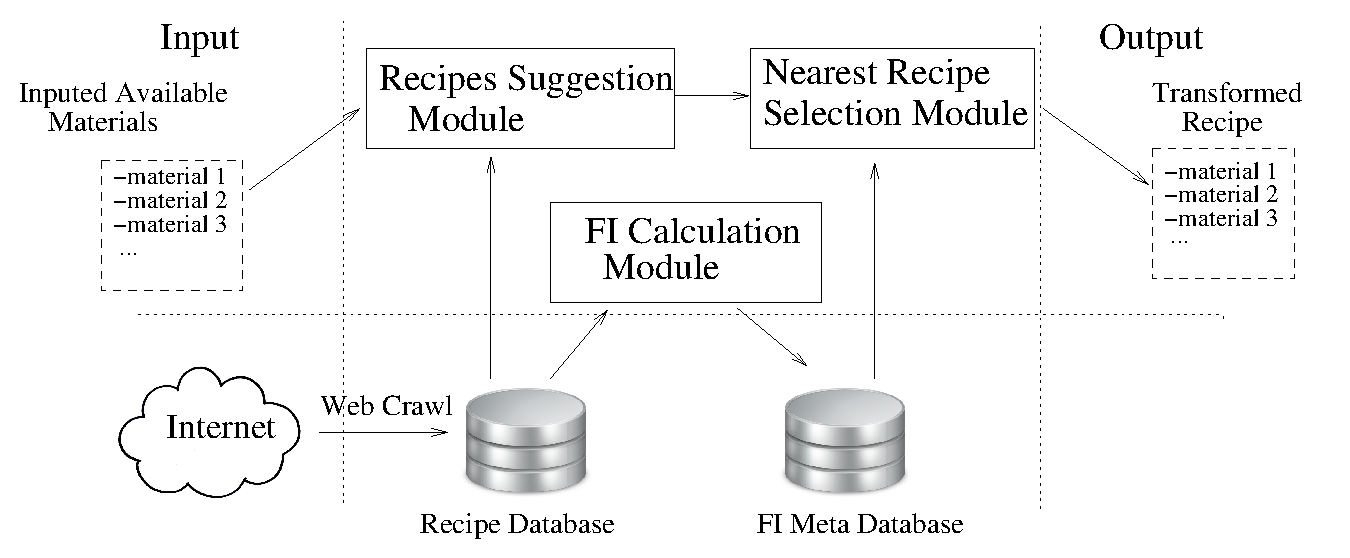
\includegraphics[scale=0.8]{system.eps} 
\caption{The System's Model with Recipe Suggestion Module, Featured Index Calculation Module and Nearest Recipe Selection Module.}
\label{fig:system-model}
\end{figure*}

\subsection{The System's Model}

\subsubsection{The Recipe Suggestion Module Based On Available Materials}

This module responds to the first function of the system, suggesting the possible recipes based on available materials inputed by the user. The input of this module is a set of available materials that the user has. It accesses the recipes database during the calculation and its output will be the list of the recipes which include most of the inputed materials. This ouput is passed to the Featured Index Calculation Module as shown in Fig.~\ref{fig:system-model}. After inputing available materials, the system will search in the recipe database for the most suitable recipes and show them in rank order. The peusedo code is shown as below. 

\begin{algorithmic}

\For{$recipe \in recipes$} 
\State $recipe.lack \gets |recipe| - |recipe \cup inputed\ materials|$
\EndFor

\State $sort\ the\ recipes\ by\ recipe.lack$

\Return $recipes$

\end{algorithmic}


\subsubsection{The Featured Index Calculation Module}

The user seclects one of the recipes recommended by the Recipe Suggestion Module. Then selects the region which they want to transform the recipe in order to have that region's taste. This module applies the region's Featured Materials Extracting Algorithm and outputs the list of Featured Index for all materials in the region then stores them in the $FI$ Meta Database as shown in Fig.~\ref{fig:system-model}. Because we are not using all of the lists to extract the featured materials, we only look at two kinds of the following materials: 

\begin{itemize}
\item The top rank $FI$ materials.

These materials are the materials which are often used in the desired region, but not in other regions. 
\item The bottom rank $FI$ materials.

These materials are the most common materials which are used in almost all regions, but with different amounts. 
	 
\end{itemize}

We use both kinds and combine them with the materials appearing in the original recipe. The result is the list of materials and their amount for the food. The output should look in the shape as follows:

\begin{itemize}
\item Onion 2     (original)
\item Lemon 1/2   (original)
\item \ldots
\item Natto 100g  (top $FI$, newly added, region's average)
\item Sugar 100g  (bottom $FI$, newly added, region's average)
\end{itemize}

Among the bottom rank $FI$ materials, we only take the materials which are already in original recipe to apply into a new recipe. Among the newly added materials we use the average amount of them in the region. The output of this module is passed to the Nearest Recipe Selection Module. 
 
\subsubsection{The Nearest Recipe Selection Module} 

The output of Featured Index Calculation Module gives us the list of materials and their amount which is suitable for the region's taste. But it doesn't mean that we could use that list to make food. If we immediately apply the list of ingredients with the associated amount, we may have a wrong solution. This is because the newly added ingredients and their associated amounts are just the mean value of ingredients in the region. In result, there is the possibility of a bad tasting food. Thus, we propose to search in the region the nearest recipe in term of ingredients and amount. Then apply the suitable ingredients and its amount in that recipe to our food.        

Consider the list of materials as a vector. We calculate the similarity between the region's recipe and the average output above. Because we currently have ingredients and their amounts, there is the problem that the unit of ingredient's amounts are different and we cannot calculate the similarity. Thus we need to normalize these units. The alternative, we propose, is taking the fraction between the recipe's amount and the average amount all over the country. This gives us the values that are unit-independent, therefore usable for the similarity calcualtion. There are various methods to calculate the similarity between two vectors~\cite{cosine,euclidean,Qian:2004:SEC:967900.968151}. Among of these methods, Cosine similarity and Euclidean distance are the most famous methods. In this paper, we use the Euclidean distance, therefore the minimum value is adapted. The details of the algorithm is shown below. $X(x_1,x_2,\ldots,x_m)$ with $m \in N $ is the list outputed by the FI Calculation Module and $Y(y_1,y_2,\ldots,y_n)$ with $n \in N $ represents a list in the lists of the specified region's recipes 


\begin{algorithmic}

\For{$ingredient \in recipe\ X $} 
\State $ x_i \gets \frac{\displaystyle amount}{\displaystyle average\ amount\ in\ the\ country}$
\EndFor

\State $min \gets \infty $
\For{$recipe \in region's\ recipes$} 
\For{$ingredient \in recipe\ Y$} 
\State $ y_i \gets \frac{\displaystyle amount}{\displaystyle average\ amount\ in\ the\ country}$
\EndFor
\State $ similarity \gets \sqrt{\displaystyle \sum^l_{i=k}{(x_i-y_i)^2}}$
\If {$ similarity < min $}
\State $ min \gets similarity $
\EndIf
\EndFor


\Return $recipes$



\end{algorithmic}

Note that though $X$ and $Y$ don't have to have the same dimensions but we only select the ingredients $i$ which appears both in $X$ and $Y$ to calculate the similarity. $x_i$ and $y_i$ in which $i \in [k,l]$, are the amounts of ingredient $i$ in $X$ and $Y$ respectively.

\section{Conclusions}

In this paper, we have presented the regional foods' features extracting algorithm and the experimental results. The experimetal results partially reflect the featured ingredients in regions. 

To show the feasibility and applicability of our algorithm, we build the cooking support system that helps cooking people transform the original recipes to have a featured taste of another regions.  

In this paper, the recipes from 7 regions of Japan are used. However, the proposed algorithm is scalable to adapt to any recipe from any region in the world. As a future work, we intent to develop a multilingual translation recipe with the function that can transform recipes between countries. 

In fact, the seasoning and non-seasoning ingredients affect the food's taste in different ways. Thus, we also develop the research in that direction, analyze food's features by applying different methods for seasiong ingredients and non-seasoning ingredients.

\bibliographystyle{plain}
\bibliography{sigproc}

\end{document}
